\documentclass[11pt]{article}

%%%%%%%%%%%%%%%%%%%%%%%%%%%%%%%%%%%%%%%%%%%%%%%%%%%%%%%%%%%%%%%
%                      Customize Header                       %
%%%%%%%%%%%%%%%%%%%%%%%%%%%%%%%%%%%%%%%%%%%%%%%%%%%%%%%%%%%%%%%

\newcommand{\assessmentTitle}{
CheckIt Assessment
}
\newcommand{\assessmentVersion}{
Version 1770955410404
}
\newcommand{\assessmentInstructions}{
Do not use any unapproved aids while taking this assessment.
Read each question carefully and be sure to show all work
in the space provided.
}

%%%%%%%%%%%%%%%%%%%%%%%%%%%%%%%%%%%%%%%%%%%%%%%%%%%%%%%%%%%%%%%
%%%%%%%%%%%%%%%%%%%%%%%%%%%%%%%%%%%%%%%%%%%%%%%%%%%%%%%%%%%%%%%



\usepackage{amsfonts,amssymb,amsmath,amsthm}
\setcounter{MaxMatrixCols}{50}
\usepackage{hyperref}
\let\oldhref\href\renewcommand{\href}[2]{\oldhref{#1}{#2}\footnote{\url{#1}}}
\usepackage[margin=1in,tmargin=2in,headheight=84pt]{geometry}
\usepackage{enumerate}
\usepackage{graphicx}
\usepackage{fancyhdr}
\usepackage{lastpage}
\pagestyle{fancy}
\fancyhf{}
\rhead{Name: \underline{\hspace{2.5in}}\\ID: \underline{\hspace{2.5in}}

\vspace{2.5em}}
\chead{\vspace{2.5em}

\fbox{\fbox{\parbox{6in}{\centering\assessmentInstructions}}}}
\lhead{\assessmentTitle \hspace{2em} \assessmentVersion

\vspace{2.5em}}
\rfoot{Page \thepage\ of \pageref{LastPage}}
\setlength{\headheight}{80pt}
\renewcommand{\headrulewidth}{0pt}


\begin{document}

\begin{enumerate}

% 

\item %%%%% SpaTeXt Commands %%%%%
\providecommand{\stxKnowl}{}\renewcommand{\stxKnowl}[1]{#1}
\providecommand{\stxOuttro}{}\renewcommand{\stxOuttro}[1]{#1}
\providecommand{\stxTitle}{}\renewcommand{\stxTitle}[1]{#1}
% Comment next line to show outtros
\renewcommand{\stxOuttro}[1]{}
%%%%%%%%%%%%%%%%%%%%%%%%%%%%
\stxKnowl{
 Simplify: \(10 - 4( 13 - |3 - 5^2| )\) 

\stxOuttro{
SOLUTION

 \(10 - 4( 13 - |3 - 5^2| )\) 

 \(= 10 - 4( 13 - |3 - 25| )\) 

 \(= 10 - 4( 13 - |-22| )\) 

 \(= 10 - 4( 13 - 22 )\) 

 \(= 10 - 4( -9 )\) 

 \(= 10 - ( -36 )\) 

 \(= \boxed{ 46 }\) 

}
}

\newpage

% 

\item %%%%% SpaTeXt Commands %%%%%
\providecommand{\stxKnowl}{}\renewcommand{\stxKnowl}[1]{#1}
\providecommand{\stxOuttro}{}\renewcommand{\stxOuttro}[1]{#1}
\providecommand{\stxTitle}{}\renewcommand{\stxTitle}[1]{#1}
% Comment next line to show outtros
\renewcommand{\stxOuttro}[1]{}
%%%%%%%%%%%%%%%%%%%%%%%%%%%%
\stxKnowl{
 Simplify the radical expression completely: 

 \(7 \sqrt[3]{ -189 }\) 

\stxOuttro{
SOLUTION

 \(7 \sqrt[3]{ -189 }\) 

 \(= 7 \cdot \sqrt[3]{ -27 \cdot 7 }\) 

 \(= 7 \cdot (-3) \sqrt[3]{ 7 }\) 

 \(= \boxed{ -21 \sqrt[3]{ 7 } }\) 

}
}

\newpage

% 

\item %%%%% SpaTeXt Commands %%%%%
\providecommand{\stxKnowl}{}\renewcommand{\stxKnowl}[1]{#1}
\providecommand{\stxOuttro}{}\renewcommand{\stxOuttro}[1]{#1}
\providecommand{\stxTitle}{}\renewcommand{\stxTitle}[1]{#1}
% Comment next line to show outtros
\renewcommand{\stxOuttro}[1]{}
%%%%%%%%%%%%%%%%%%%%%%%%%%%%
\stxKnowl{
 Simplify: \(\displaystyle \left( \frac{ -3 a^{-5} b^{3} c^{0} }{ a^{-4} b^{4} c^{2} } \right)^{ -3 }\) 

\stxOuttro{
SOLUTION

 \(\displaystyle \left( \frac{ -3 a^{-5} b^{3} c^{0} }{ a^{-4} b^{4} c^{2} } \right)^{ -3 }\) 

 \(= \left( -3 a^{-1} b^{-1} c^{-2} \right)^{-3}\) 

 \(= (-3)^{-3} a^{3} b^{3} c^{6}\) 

 \(= \boxed{ - \frac{a^{3}b^{3}c^{6}}{27} }\) 

}
}

\newpage

% 

\item %%%%% SpaTeXt Commands %%%%%
\providecommand{\stxKnowl}{}\renewcommand{\stxKnowl}[1]{#1}
\providecommand{\stxOuttro}{}\renewcommand{\stxOuttro}[1]{#1}
\providecommand{\stxTitle}{}\renewcommand{\stxTitle}[1]{#1}
% Comment next line to show outtros
\renewcommand{\stxOuttro}[1]{}
%%%%%%%%%%%%%%%%%%%%%%%%%%%%
\stxKnowl{
 Simplify: \((-3 \, x^{2} + 3 \, x + 9) - (3 \, x^{2} - 4 \, x - 7)\) 

\stxOuttro{
SOLUTION

 \((-3 \, x^{2} + 3 \, x + 9) - (3 \, x^{2} - 4 \, x - 7)\) 

 \(= -3x^2+3x+9-3x^2+4x+7\) 

 \(= -3x^2-3x^2+3x+4x+9+7\) 

 \(= \boxed{ -6 \, x^{2} + 7 \, x + 16 }\) 

}
}

\newpage

% 

\item %%%%% SpaTeXt Commands %%%%%
\providecommand{\stxKnowl}{}\renewcommand{\stxKnowl}[1]{#1}
\providecommand{\stxOuttro}{}\renewcommand{\stxOuttro}[1]{#1}
\providecommand{\stxTitle}{}\renewcommand{\stxTitle}[1]{#1}
% Comment next line to show outtros
\renewcommand{\stxOuttro}[1]{}
%%%%%%%%%%%%%%%%%%%%%%%%%%%%
\stxKnowl{
 Simplify: \((3u - 4v)(9u^2 + 12uv + 16v^2)\) 

\stxOuttro{
SOLUTION

 \((3u - 4v)(9u^2 + 12uv + 16v^2)\) 

 \(= 3u(9u^2 + 12uv + 16v^2) - 4v(9u^2 + 12uv + 16v^2)\) 

 \(= 27u^3 + 36u^2v + 48uv^2 - 36u^2v - 48uv^2 - 64v^3\) 

 \(= \boxed{ 27u^3 - 64v^3 }\) 

}
}

\newpage

% 

\item %%%%% SpaTeXt Commands %%%%%
\providecommand{\stxKnowl}{}\renewcommand{\stxKnowl}[1]{#1}
\providecommand{\stxOuttro}{}\renewcommand{\stxOuttro}[1]{#1}
\providecommand{\stxTitle}{}\renewcommand{\stxTitle}[1]{#1}
% Comment next line to show outtros
\renewcommand{\stxOuttro}[1]{}
%%%%%%%%%%%%%%%%%%%%%%%%%%%%
\stxKnowl{
 Simplify: \(\displaystyle \frac{ 12 \, x^{4} - 19 \, x^{3} + 17 \, x^{2} - x + 8 }{ 3 \, x - 1 }\) 

\stxOuttro{
SOLUTION

 \(\begin{array}{r} 4 \, x^{3} - 5 \, x^{2} + 4 \, x + 1 \\ 3 \, x - 1 \overline{ ) 12 \, x^{4} - 19 \, x^{3} + 17 \, x^{2} - x + 8 } \\ \underline{ -( 12 \, x^{4} - 4 \, x^{3} ) } \\\\ -15 \, x^{3} + 17 \, x^{2} - x + 8 \\ \underline{ -( -15 \, x^{3} + 5 \, x^{2} ) } \\\\ 12 \, x^{2} - x + 8 \\ \underline{ -( 12 \, x^{2} - 4 \, x ) } \\\\ 3 \, x + 8 \\ \underline{ -( 3 \, x - 1 ) } \\\\ 9 \end{array}\) 

 \(= \boxed{ 4 \, x^{3} - 5 \, x^{2} + 4 \, x + 1 + \frac{9}{3 \, x - 1} }\) 

}
}

\newpage

% 

\item %%%%% SpaTeXt Commands %%%%%
\providecommand{\stxKnowl}{}\renewcommand{\stxKnowl}[1]{#1}
\providecommand{\stxOuttro}{}\renewcommand{\stxOuttro}[1]{#1}
\providecommand{\stxTitle}{}\renewcommand{\stxTitle}[1]{#1}
% Comment next line to show outtros
\renewcommand{\stxOuttro}[1]{}
%%%%%%%%%%%%%%%%%%%%%%%%%%%%
\stxKnowl{
 Solve: \(12 - 4(2x - 2) = 2(3x - 25)\) 

\stxOuttro{
SOLUTION

 \(12 - 4(2x - 2) = 2(3x - 25)\) 

 \(12 - 8x + 8 = 6x - 50\) 

 \(20 - 8x = 6x - 50\) 

 \(20 = 14x - 50\) 

 \(70 = 14x\) 

 \(\boxed{ x = 5 }\) 

}
}

\newpage

% 

\item %%%%% SpaTeXt Commands %%%%%
\providecommand{\stxKnowl}{}\renewcommand{\stxKnowl}[1]{#1}
\providecommand{\stxOuttro}{}\renewcommand{\stxOuttro}[1]{#1}
\providecommand{\stxTitle}{}\renewcommand{\stxTitle}[1]{#1}
% Comment next line to show outtros
\renewcommand{\stxOuttro}[1]{}
%%%%%%%%%%%%%%%%%%%%%%%%%%%%
\stxKnowl{
 Solve: \(\displaystyle \frac{3}{8}x - \frac{1}{2} = 4\) 

\stxOuttro{
SOLUTION

 \(\displaystyle \frac{3}{8}x - \frac{1}{2} = 4\) 

 \(8 \left( \frac{3}{8}x - \frac{1}{2} = 4 \right)\) 

 \(3x - 4 = 32\) 

 \(3x = 36\) 

 \(x = 12\) 

 \(\boxed{ x = 12 }\) 

}
}

\newpage

% 

\item %%%%% SpaTeXt Commands %%%%%
\providecommand{\stxKnowl}{}\renewcommand{\stxKnowl}[1]{#1}
\providecommand{\stxOuttro}{}\renewcommand{\stxOuttro}[1]{#1}
\providecommand{\stxTitle}{}\renewcommand{\stxTitle}[1]{#1}
% Comment next line to show outtros
\renewcommand{\stxOuttro}[1]{}
%%%%%%%%%%%%%%%%%%%%%%%%%%%%
\stxKnowl{
 Solve for \(x\): \(dx - ey = f\) 

\stxOuttro{
SOLUTION

 \(dx - ey = f\) 

 \(dx = f + ey\) 

 \(\boxed{ x = \frac{f + ey}{d} }\) 

}
}

\newpage

% 

\item %%%%% SpaTeXt Commands %%%%%
\providecommand{\stxKnowl}{}\renewcommand{\stxKnowl}[1]{#1}
\providecommand{\stxOuttro}{}\renewcommand{\stxOuttro}[1]{#1}
\providecommand{\stxTitle}{}\renewcommand{\stxTitle}[1]{#1}
% Comment next line to show outtros
\renewcommand{\stxOuttro}[1]{}
%%%%%%%%%%%%%%%%%%%%%%%%%%%%
\stxKnowl{
 A moving truck costs \$\(48.00\) per day plus \$\(0.40\) per mile driven. If Dana has \$\(167.20\) for a one-day rental, how many miles can they drive? 

\stxOuttro{
SOLUTION

 \(167.20 - 48.00 = 119.20\) 

 \(\frac{119.20}{0.40} = 298\) 

 \(\boxed{ 298 \text{ miles} }\) 

}
}

\newpage

% 

\item %%%%% SpaTeXt Commands %%%%%
\providecommand{\stxKnowl}{}\renewcommand{\stxKnowl}[1]{#1}
\providecommand{\stxOuttro}{}\renewcommand{\stxOuttro}[1]{#1}
\providecommand{\stxTitle}{}\renewcommand{\stxTitle}[1]{#1}
% Comment next line to show outtros
\renewcommand{\stxOuttro}[1]{}
%%%%%%%%%%%%%%%%%%%%%%%%%%%%
\stxKnowl{
 Graph and identify the slope and intercepts of the function: \(f(x) = \displaystyle{ \frac{2}{7} }x + 2\) 

 \begin{tikzpicture}[scale=0.4] \draw[help lines, color=gray!50] (-10,-10) grid (10,10); \draw[<->, thick] (-10.5,0)--(10.5,0) node[right]{$x$}; \draw[<->, thick] (0,-10.5)--(0,10.5) node[above]{$y$}; \end{tikzpicture} 

\stxOuttro{
SOLUTION

 \(\text{Slope: } m = \frac{2}{7}\) 

 \(\text{y-intercept: } (0, 2)\) 

 \(\text{x-intercept: } (-7, 0)\) 

 \begin{tikzpicture}[scale=0.4] \draw[help lines, color=gray!50] (-10,-10) grid (10,10); \draw[<->, thick] (-10.5,0)--(10.5,0) node[right]{$x$}; \draw[<->, thick] (0,-10.5)--(0,10.5) node[above]{$y$}; \begin{scope} \clip (-10,-10) rectangle (10,10); \draw[<->, ultra thick, blue, domain=-11:11, samples=2] plot (\x, {0.2857142857142857*\x + 2.0}); \end{scope} \fill[red] (-7,0) circle (0.3); \fill[red] (0,2) circle (0.3); \end{tikzpicture} 

}
}

\newpage

% 

\item %%%%% SpaTeXt Commands %%%%%
\providecommand{\stxKnowl}{}\renewcommand{\stxKnowl}[1]{#1}
\providecommand{\stxOuttro}{}\renewcommand{\stxOuttro}[1]{#1}
\providecommand{\stxTitle}{}\renewcommand{\stxTitle}[1]{#1}
% Comment next line to show outtros
\renewcommand{\stxOuttro}[1]{}
%%%%%%%%%%%%%%%%%%%%%%%%%%%%
\stxKnowl{
 Given \(g(x) = x^2 - 6x + 8\), find each of the following. 

\begin{enumerate}
\item
\stxKnowl{
 \(g(-1)\) 

\stxOuttro{
 \(g(-1) = (-1)^2 - 6(-1) + 8\) 

 \(= 1 + 6 + 8\) 

 \(= \boxed{ 15 }\) 

}
}

\item
\stxKnowl{
 \(g(0)\) 

\stxOuttro{
 \(g(0) = (0)^2 - 6(0) + 8\) 

 \(= \boxed{ 8 }\) 

}
}

\item
\stxKnowl{
 \(g(x+h)\) 

\stxOuttro{
 \(g(x+h) = (x+h)^2 - 6(x+h) + 8\) 

 \(= \boxed{ x^2 + 2xh + h^2 - 6x - 6h + 8 }\) 

}
}

\end{enumerate}
}

\newpage

% 

\item %%%%% SpaTeXt Commands %%%%%
\providecommand{\stxKnowl}{}\renewcommand{\stxKnowl}[1]{#1}
\providecommand{\stxOuttro}{}\renewcommand{\stxOuttro}[1]{#1}
\providecommand{\stxTitle}{}\renewcommand{\stxTitle}[1]{#1}
% Comment next line to show outtros
\renewcommand{\stxOuttro}[1]{}
%%%%%%%%%%%%%%%%%%%%%%%%%%%%
\stxKnowl{
 For each graph below, determine whether it represents a function and identify the domain and range. 

\begin{enumerate}
\item
\stxKnowl{
 \begin{tikzpicture}[scale=0.35] \draw[step=1cm, gray!40, very thin] (-10,-10) grid (10,10); \draw[thick, <->] (-10.5,0) -- (10.5,0) node[right] {$x$}; \draw[thick, <->] (0,-10.5) -- (0,10.5) node[above] {$y$}; \foreach \x in {-10,-8,...,10} \draw (\x, 0.1) -- (\x, -0.1) node[below] {\tiny $\x$}; \foreach \y in {-10,-8,...,10} \draw (0.1, \y) -- (-0.1, \y) node[left] {\tiny $\y$}; \draw[ultra thick, blue, <->, domain=-6.741657386773941:0.7416573867739413, samples=100] plot (\x, {0.500000000000000*(\x - -3)^2 + 3}); \end{tikzpicture} 

\stxOuttro{
Solution

\begin{itemize}
\item
Domain: \((-\infty, \infty)\)

\item
Range: \([3, \infty)\)

\item
Function

\end{itemize}
}
}

\item
\stxKnowl{
 \begin{tikzpicture}[scale=0.35] \draw[step=1cm, gray!40, very thin] (-10,-10) grid (10,10); \draw[thick, <->] (-10.5,0) -- (10.5,0) node[right] {$x$}; \draw[thick, <->] (0,-10.5) -- (0,10.5) node[above] {$y$}; \foreach \x in {-10,-8,...,10} \draw (\x, 0.1) -- (\x, -0.1) node[below] {\tiny $\x$}; \foreach \y in {-10,-8,...,10} \draw (0.1, \y) -- (-0.1, \y) node[left] {\tiny $\y$}; \draw[ultra thick, blue, <->, domain=-3.9282032302755088:9.928203230275509, samples=100] plot ({0.250000000000000*(\x - 3)^2 + -2}, \x); \end{tikzpicture} 

\stxOuttro{
Solution

\begin{itemize}
\item
Domain: \([-2, \infty)\)

\item
Range: \((-\infty, \infty)\)

\item
Not a function

\end{itemize}
}
}

\end{enumerate}
}

\newpage

% 

\item %%%%% SpaTeXt Commands %%%%%
\providecommand{\stxKnowl}{}\renewcommand{\stxKnowl}[1]{#1}
\providecommand{\stxOuttro}{}\renewcommand{\stxOuttro}[1]{#1}
\providecommand{\stxTitle}{}\renewcommand{\stxTitle}[1]{#1}
% Comment next line to show outtros
\renewcommand{\stxOuttro}[1]{}
%%%%%%%%%%%%%%%%%%%%%%%%%%%%
\stxKnowl{
 Given the graph of the function \(f\) below, find each of the following. 

 \begin{tikzpicture}[scale=0.35] \draw[step=1cm, gray!40, very thin] (-10,-10) grid (10,10); \draw[thick, <->] (-10.5,0) -- (10.5,0) node[right] {$x$}; \draw[thick, <->] (0,-10.5) -- (0,10.5) node[above] {$y$}; \foreach \x in {-10,-8,...,10} \draw (\x, 0.1) -- (\x, -0.1) node[below] {\tiny $\x$}; \foreach \y in {-10,-8,...,10} \draw (0.1, \y) -- (-0.1, \y) node[left] {\tiny $\y$}; \draw[ultra thick, blue, <->, domain=-4.741657386773941:2.7416573867739413, samples=100] plot (\x, {1*(\x - -1)^2 + -4}); \end{tikzpicture} 

\begin{itemize}
\item
(a) \(f(0)\)

\item
(b) \(f(1)\)

\item
(c) \(f(-3)\)

\item
(d) Find \(x\) where \(f(x) = -4\)

\end{itemize}
\stxOuttro{
Solution

\begin{itemize}
\item
(a) \(-3\)

\item
(b) \(0\)

\item
(c) \(0\)

\item
(d) \(x = -1\)

\end{itemize}
}
}

\newpage

% 

\item %%%%% SpaTeXt Commands %%%%%
\providecommand{\stxKnowl}{}\renewcommand{\stxKnowl}[1]{#1}
\providecommand{\stxOuttro}{}\renewcommand{\stxOuttro}[1]{#1}
\providecommand{\stxTitle}{}\renewcommand{\stxTitle}[1]{#1}
% Comment next line to show outtros
\renewcommand{\stxOuttro}[1]{}
%%%%%%%%%%%%%%%%%%%%%%%%%%%%
\stxKnowl{
 Find the equation of the line parallel to \(5x - 8y = 8\) and passing through \((-1, -1)\). 

\stxOuttro{
Solution

Slope:

 \(5x - 8y = 8\) 

 \(-8y = -5x + 8\) 

 \(y = \frac{5}{8}x + -1\) 

 \(m = \frac{5}{8}\) 

Y-intercept:

 \(y = mx + b\) 

 \(-1 = \frac{5}{8}(-1) + b\) 

 \(-1 = -\frac{5}{8} + b\) 

 \(b = -\frac{3}{8}\) 

 \(\boxed{ y = \frac{5}{8}x - \frac{3}{8} }\) 

}
}

\newpage

% 

\item %%%%% SpaTeXt Commands %%%%%
\providecommand{\stxKnowl}{}\renewcommand{\stxKnowl}[1]{#1}
\providecommand{\stxOuttro}{}\renewcommand{\stxOuttro}[1]{#1}
\providecommand{\stxTitle}{}\renewcommand{\stxTitle}[1]{#1}
% Comment next line to show outtros
\renewcommand{\stxOuttro}[1]{}
%%%%%%%%%%%%%%%%%%%%%%%%%%%%
\stxKnowl{
 A particular search engine assigns a ranking to a webpage based on the number of links that direct users to the webpage. The ranking of a webpage is given by the function below, where \(n\) represents the number of links that direct users to it. How many links will be needed to obtain a page ranking of 10? 

 \(R(n) = \frac{1}{9}n + 3\) 

\stxOuttro{
Solution

 \(10 = \frac{1}{9}n + 3\) 

 \(7 = \frac{1}{9}n\) 

 \(63 = n\) 

 \(\boxed{ 63 \text{ links} }\) 

}
}

\newpage

% 

\item %%%%% SpaTeXt Commands %%%%%
\providecommand{\stxKnowl}{}\renewcommand{\stxKnowl}[1]{#1}
\providecommand{\stxOuttro}{}\renewcommand{\stxOuttro}[1]{#1}
\providecommand{\stxTitle}{}\renewcommand{\stxTitle}[1]{#1}
% Comment next line to show outtros
\renewcommand{\stxOuttro}[1]{}
%%%%%%%%%%%%%%%%%%%%%%%%%%%%
\stxKnowl{
 Solve the system of equations. 

 \(\begin{cases} x - y = -1 \\ x + y = -7 \end{cases}\) 

\stxOuttro{
Solution

 \(x - y = -1 \to x = y - 1\) 

Substitute:

 \((y - 1) + y = -7\) 

 \(2y - 1 = -7\) 

 \(2y = -6\) 

 \(y = -3\) 

Back-substitute:

 \(x = -3 + (-1)\) 

 \(x = -4\) 

 \(\boxed{ (-4, -3) }\) 

}
}

\newpage

% 

\end{enumerate}

\end{document}